%\documentclass[main.tex]{subfiles}
%\begin{document}

\section{Facility Description}

The CHARM facility consists of a main test area (also referred to as target area), 2 control rooms and a buffer-area for storage \footnote{A more detailed description of the facility can be found in the safety file \cite{charm_safety_file}.}. A layout drawing of the T8 beam-line and surrounding areas is shown in figure \ref{fig:irrads_layout}, and a photo of the test area is shown in \ref{fig:test_area_photo}. The main (larger) control room is dedicated to monitoring the facility and has space for users to make dry-runs of their test set-up, whereas the technical-locale is where the control and monitoring equipment for the users is installed during their tests. A separate platform outside the control room is available for testing large devices (full sized racks and large equipment) which connects directly with the control room for dry-testing. All the connections and cabling (including length) within the control match exactly those used between the test area and technical-locale, as to keep the dry-run set-up configuration exactly the same as with the real tests.  \\

To perform a test, the users device is installed on a rack and moved to the test positions using an automated conveyor system (AVT). The test positions are shown in figure \ref{fig:fluka_test_positions}.  The cabling for the test device is placed into a 'cable-order-chain' attached to a rail system and is moved in to place together with the conveyor. Figure \ref{fig:cable_chain} shows how the cables are arranged. Inside the test area there is a patch-panel with an array of different connections for the user to connect their equipment. These connections lead directly to a patch-panel inside the technical locale. A list of available cables and connectors can be found on the CHARM website: \url{http://charm.web.cern.ch/CHARM/Cables.php} \\

During operation the beam is directed on one of three targets; copper, aluminium and 'aluminium with holes'. By choosing different targets, the intensity of the radiation field can be varied, with the copper target generally giving the highest dose and particle fluences, and the 'aluminmium with holes' target giving the least dose compared to the other targets. For in beam measurements it is possible to run without target, so one can test in a 24 GeV proton field. \\

There are four layers of shielding installed in the middle of the area which can be moved in and out of place to tailor the radiation field. The outer two layers of 20cm thick concrete surround two layers of 20cm thick iron in a 'sandwich' arrangement. The 'concrete-iron-iron-concrete' layout is referred to as 'CIIC' for the facility configuration, where partial shielding and running without any shielding at referred to as 'CIOO' (concrete-iron-open-open) and 'OOOO' (all four open). \\

Within the test area there are a number of different positions one can place test equipment in CHARM, which can either be directly in the proton beam, behind shielding or at various angles and distances from the target. These are either at the designated test positions or at the Montrac positions. By varying the target, shielding and position of the test device, a large number of radiation fields can be achieved. These are described in detail in chapter 3. \\

\begin{figure}[ht!]
	\centering
	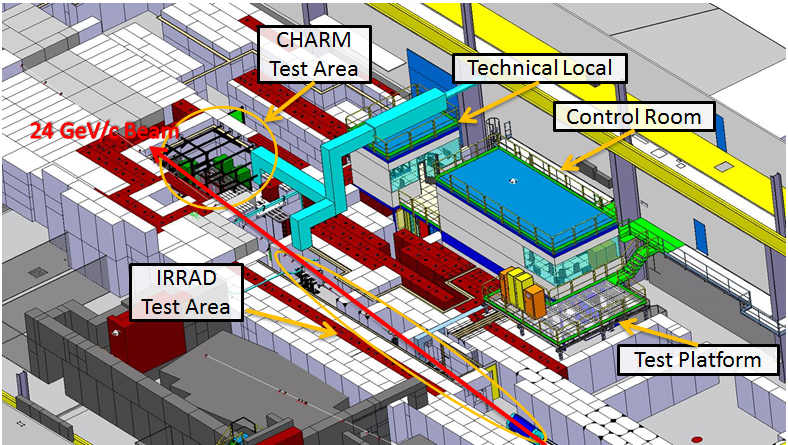
\includegraphics[width=0.8\textwidth]{./images/charm_overall_ann}
	\caption{A screen-shot from the 3D Catia drawing of the IRRAD and CHARM facility, showing the different areas.}
	\label{fig:irrads_layout}
\end{figure}

\begin{figure}[!ht]
	\centering
	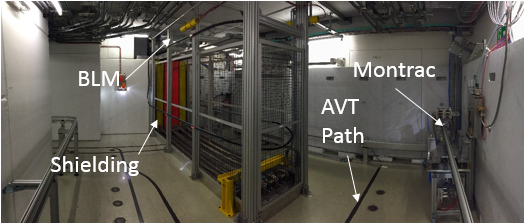
\includegraphics[width=\textwidth]{./images/test_area_photo_ann}
	\caption{A photo of the test area. The moveable shielding is in the centre of the photo, with the target behind.}
	\label{fig:test_area_photo}
\end{figure}

\begin{figure}[ht!]
	\centering
	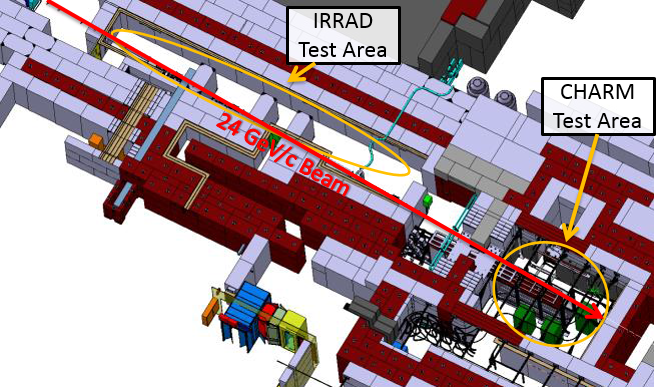
\includegraphics[width=0.8\textwidth]{./images/irrad2}
	\caption{A screen-shot of the 3D Catia drawings for the T8 beam-line on the East Area hall showing the position of the IRRAD and CHARM facilities along the T8 beam-line.}
	\label{fig:t8_screenshot}
\end{figure}

\begin{figure}[!ht]
	\centering
	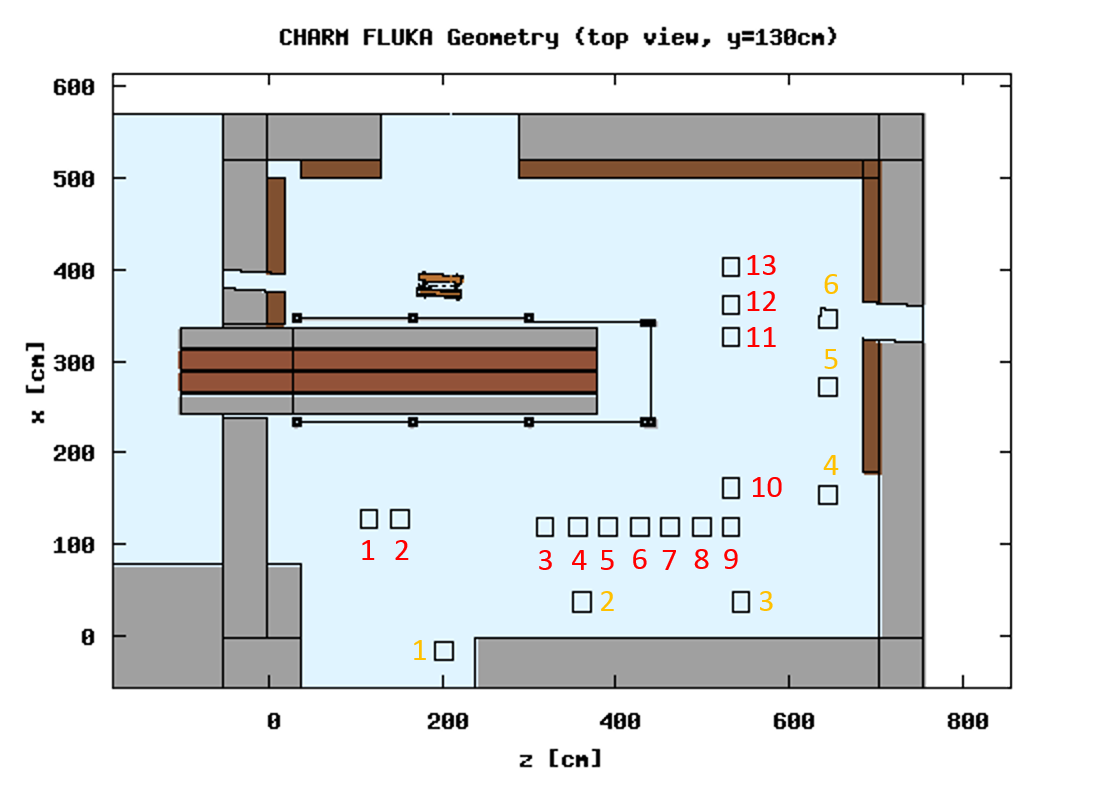
\includegraphics[width=0.8\textwidth]{./images/test_pos_new_ann}
	\caption{A screen-shot showing the test positions in the FLUKA geometry, cut at beam-height. The rack positions are numbered in red, and the Montrac test positions are numbered in yellow.}
	\label{fig:fluka_test_positions}
\end{figure}

\clearpage
\subsection{Facility Configuration}

There are a number of possible ways to change the radiation field within the test area depending on the requirements of the users and the desired test environment. Below is a list of the options.

\begin{description}
\item[Targets] \hfill \\
There are 3 targets for use in the test area; copper, aluminium and aluminium with holes. The first 2 are solid metal, however the third is made from machined disks of aluminium with cuts made through the centre, reducing the effective density along with middle by a factor 2, leading to less beam interaction. These are referred to as 'cp', 'al' and 'alh' respectively.

\item[Shielding] \hfill \\
Between the test positions and target inside the test area, there are 4 movable shielding plates, made of either concrete ('C') or iron ('I'). The configuration of the shielding is referred to in the calculations as the order starting closest to the target and going further away. An example is 'CIIC', which means all shielding is in place, alternatively there are 'CIOO' which means half shielding, and 'OOOO' which means no shielding being used. 

\item[Test Positions] \hfill \\
%to do! update with 13 new positions
These are the 'rack' test positions, for which a conveyor system will be used to move the racks filled with the test electronics. There are a total of 13 possible rack positions, which will be referred to as 'r1' to 'r13'. These are in the mixed-field. The positions shown in figure \ref{fig:fluka_test_positions} and the coordinates relative to the FLUKA geometry are described in the appendix in table \ref{tab:test_positions}.

\item[Beam Conditions] \hfill \\
The beam extracted from the PS can be altered in a number of ways to suit the needs of the users. Firstly considering the effective beam intensity reaching the facility, the spill size and frequency can be altered. This can be varied from around 1E11 up to 5E11 per spill with up to 6 spills per super-cycle, giving around a factor 30 range in intensity for the users. More details on the beam conditions are given in the following section. \\
\end{description}

\noindent In addition to the above, there are other special test positions available: \\

\begin{description}
\item[Montrac Positions] \hfill \\
% to do! 
These are positions along the Montrac rail system where the shuttle can stop and one can leave the equipment to be irradiated. There are fewer positions that the usual test locations, but adds additional positions for smaller equipment that can be run in parallel with the large racks. A photo of the Montrac test location is shown in figure \ref{fig:montrac_testbox}.

\item[In-beam Position] \hfill \\
In addition to the Montrac positions, it is possible to stop the shuttle directly in beam and leave equipment for testing.
\end{description}

\begin{figure}
\centering
\begin{subfigure}{.5\textwidth}
  \centering
  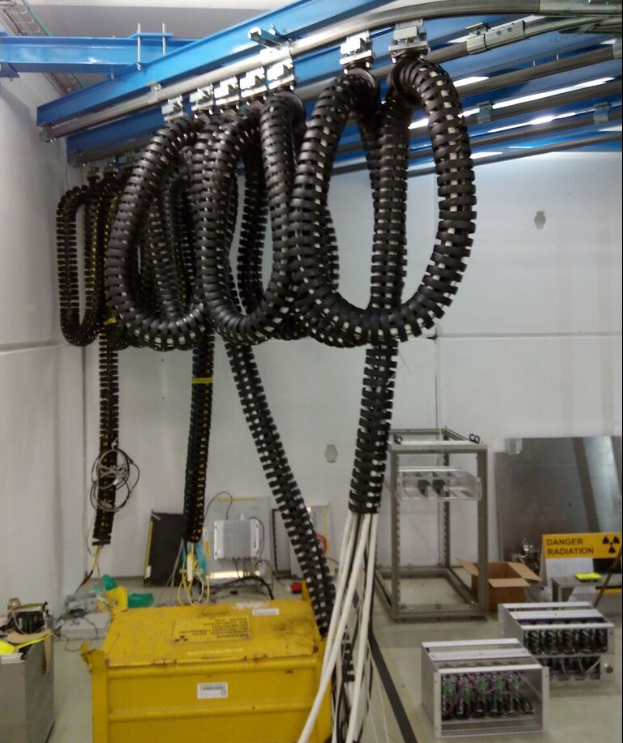
\includegraphics[width=.9\linewidth]{./images/cable_chain_storage}
  \caption{}
  \label{fig:cable_chain1}
\end{subfigure}%
\begin{subfigure}{.5\textwidth}
  \centering
  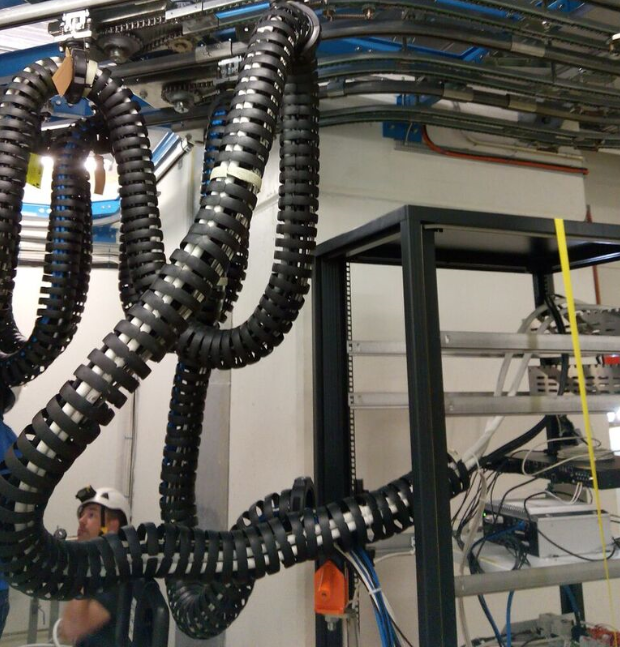
\includegraphics[width=.9\linewidth]{./images/cable_chain_to_rack}
  \caption{}
  \label{fig:cable_chain2}
\end{subfigure}
\caption{A photo of the cable-order-chain used to keep all the user cables together, and runs on a rail system making it easy to manipulate a potentially heavy mass of cables. Photo (a) shows the cable within the storage area, and photo (b) shows a test rack being connected to the cables.}
\label{fig:cable_chain}
\end{figure}

\begin{figure}[!ht]
	\centering
	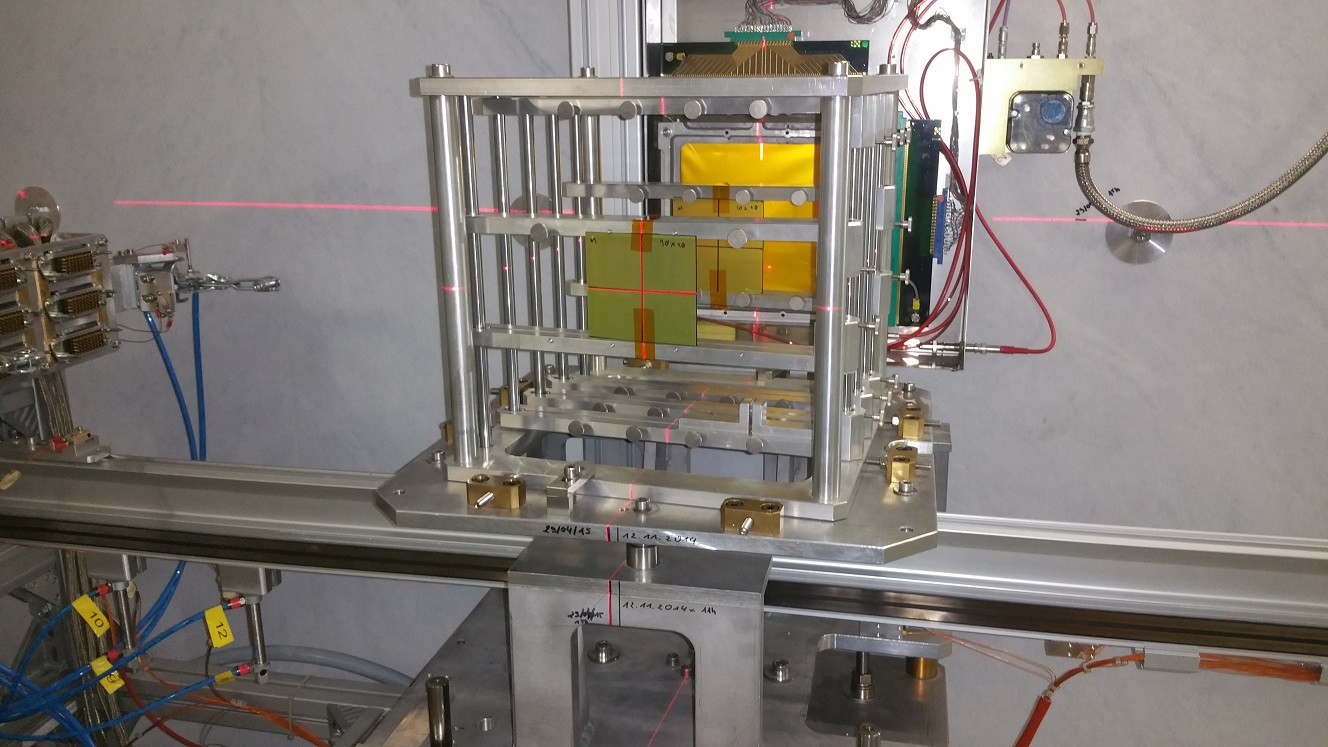
\includegraphics[width=0.8\textwidth]{./images/montrac_testbox2}
	\caption{A photo of the Montrac test location with the test rack in place, ready for in-beam tests.}
	\label{fig:montrac_testbox}
\end{figure}


% beatch file in appendix

\clearpage
\subsection{Beam Instrumentation}
For monitoring the beam reaching the IRRAD and CHARM test facilities, there are a number of instruments that can be used to measure the beam intensity, position and size. All the available monitors are shown in figure \ref{fig:t8_instrumets}. The instrumentation falls into 2 categories; \textbf{intensity monitoring}, and \textbf{position and beam size monitoring}. \\

\subsubsection{Beam Intensity Monitoring}

The beam intensity can be measured using either of the secondary emission counters (SEC1 and SEC2) or the ionisation chamber (IC). \textbf{To determine the number of protons reaching the target (POT) at CHARM, the SEC1 detector is to be used as the reference.} This detector is calibrated using the 'fast beam current transformer' (BCT) placed up-stream, just after the point of extraction from the PS. A cross-check is also made using activation foils. \\

During the SEC1 calibration tests \cite{pozzi2015} a calibration factor of 1.84E7 protons per SEC1 count was found using an activation foil method. This is the value that will be used to normalise experimental results to compare with the FLUKA calculations. \\

The SEC2 can also be used to measure the POT, however as this detector is positioned after the IRRAD facility, the signal can be influenced by sampled placed in beam at IRRAD. This has been observed during operation and can give misleading beam intensity measurements (reference), therefore it is recommended to use the SEC1 for POT calculations. The data from the SEC1, SEC2 and IC are all continuously logged in TIMBER. The variable names are listed in table \ref{tab:beam_instruments}. \\

\subsubsection{Beam Position and Size Monitoring}

The position of the beam can be measured as it passes through IRRAD using the 'beam position monitors' (BPM) (\url{https://ps-irrad.web.cern.ch/irrad/bpm.php}) and with the 'beam TV' (BTV) or 'multi-wire proportional chamber' (MWPC) as it passes CHARM. The BTV is only used to verify the beam position is correct after changes on the T8 beam-line. During operation the MWPC is used to monitor the beam shape and position. The detector is placed at the back of CHARM, just behind the Montrac test position. The data is logged in TIMBER under the variable names described in table \ref{tab:beam_instruments}. \\


\begin{table}[h!]
	\begin{center}
	\begin{tabular}{l|l}
	Detector & TIMBER Variable Name \\ 
	\hline 
	\hline
	SEC1 &  MSC01.ZT8.107:COUNTS \\ 
	SEC2 & MSC02.ZT8.125:COUNTS  \\ 
	IC & ION01.ZT8.124:COUNTS \\ 
	MWPC (x) & MWPC.ZT8.135:PROFILE\_H \\ 
	MWPC (y) & MWPC.ZT8.135:PROFILE\_V \\ 
	\end{tabular}
	\end{center}
	\caption{A table of the variable names as used in the logging database for the various beam instruments. The 'ZT8' refers to the T8 beam-line, and the number proceeding it refers to the distance of the detector to the beam extraction from the PS.}
	\label{tab:beam_instruments}
\end{table}

\begin{figure}[!ht]
	\centering
	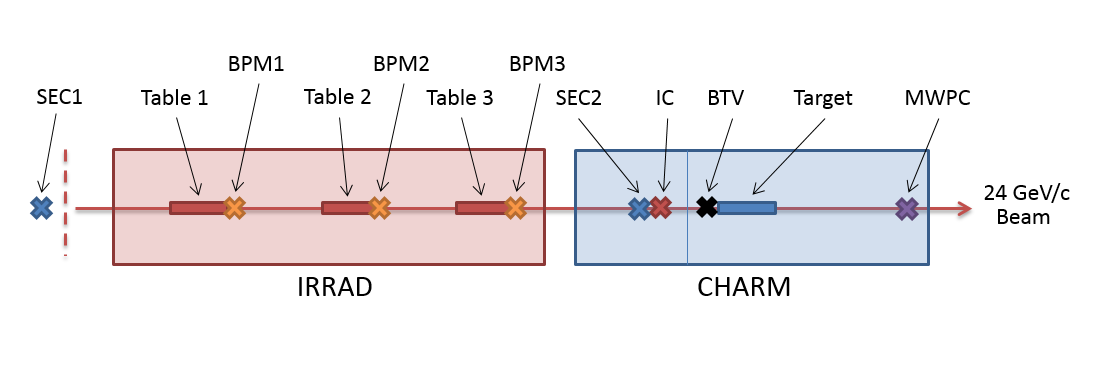
\includegraphics[width=\textwidth]{./images/beam_layout}
	\caption{A diagram of the beam instrumentation for the T8 beam-line.}
	\label{fig:t8_instrumets}
\end{figure}

\subsection{Beam Specification}

The CHARM facility receives a 24 GeV/c proton beam extracted from the CERN proton-synchrotron (PS), which is directed along the T8 beam-line in the PS East-Area Hall towards CHARM. The beam structure is in 'spills' (or bunches) of length 350ms, separated by 1.2 seconds and ordered in a 'super-cycle' usually of around 30 spills. This gives the beam a 'burst' like nature, as opposed to a constant beam without interruption. Each user of the beam is allocated a specific spill (or several spills) and these are extracted individually to the respective beam-lines. An example of how the spills are typically arranged can be seen in figure \ref{fig:ps_vista}. \\  

The beam conditions for the T8 beam-line can vary based on the different parameters used from extraction down to the magnets preceding the IRRAD facility. For the cases when the target is being used, the beam will be focused on the target, with a FWHM of around 3cm. For direct irradiation in the beam, it is possible to enlarge the beam up to a FWHM of 10cm. More information about the  beam parameters and conditions can be found in the T8 beam specification document \cite{Gatignon2013}. A summary of the usual beam conditions is shown in the next section. A detailed report on the beam characteristics during the enlarged beam size has been made available on EDMS \cite{charmblown}.\\

\begin{figure}[!ht]
	\centering
	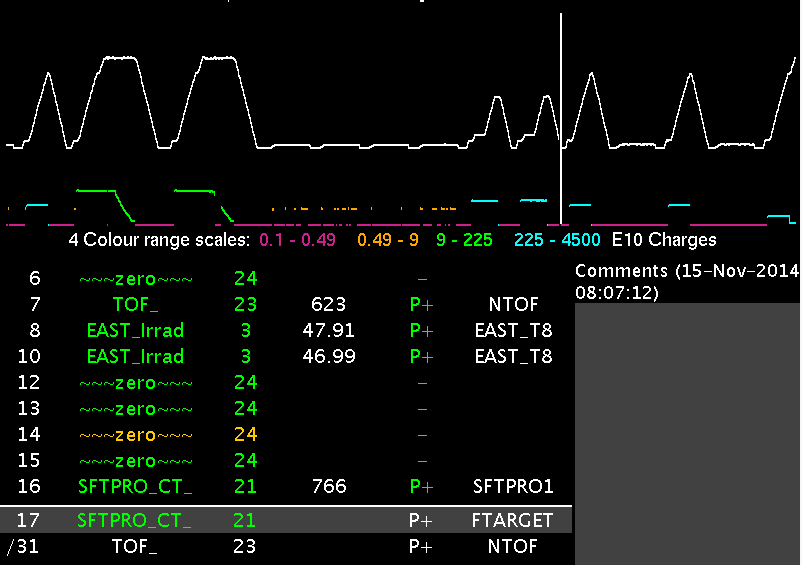
\includegraphics[width=0.6\textwidth]{./images/vistar_example}
	\caption{A screen-shot of the PS VISTAR page, giving live information about the beam extracted from the CERN PS. In this example, CHARM is receiving 2 spills (numbers 8 and 10) from a super-cycle of length 31 spills. The intensity measured at extraction in this case is around 4.7E11 protons per spill.}
	\label{fig:ps_vista}
\end{figure}

\subsection{Operating Conditions}

During the initial test period in October 2014, an analysis was made of the average beam intensity. It was possible to determine the average spill size and frequency, which can be used to make an estimate for the number of POT impinging the target over a set period. It was found that the average intensity seen on the SEC1 was 3.1E11 protons per spill. It was also noted that there was typically 3 spills per minute, which gives an average of around 1.8E10 protons per second, or 1.5E15 protons per day of running. This assumes no break in operation and no changes in the beam conditions. Therefore, to use a reasonable scaling value for the remaining document, \textbf{1.5E15 protons per day} will be assumed when normalising datasets, and will be referred to hereafter as the nominal operation conditions. \\

During the same period it was noted that the spill frequency can be varied from 1 to 6 spills per minute, and the spill intensity can vary from 1.5E11 to around a maximum of 4.0E11 protons per spill. This gives the lower and upper running limits of around 2.1E14 to 2.3E15 protons per day respectively. \\

The beam size for irradiation with the target uses the normal beam conditions from the PS, which gives a beam-size of around 1 to 2cm FWHM at the target. For in beam tests, it is possible to request the 'blown-up' beam setting from the PS operators. The reference for this was set during tests on 01/06/2015, and a beam of 8cm FWHM in the horizontal plane, and 12cm FWHM in the vertical was achieved. A plot of this on the MWPC is shown in figure \ref{fig:beam_reference2}. The values for the beam reference can be found in table \ref{tab:mwpc_reference_values}. \\

The beam profile on the BPM1 was analysed for the test periods over November and December 2014 and an average made over all channels in the x and y planes. It was seen to have a Gaussian distribution, with a FWHM of 14.6mm and 10.7mm in x and y respectively. The profile differed slightly for BPM2 where the beam was larger in the y plane, with a FWHM of 11.5mm and 14.1mm in x and y respectively. \\

%to do! update with the reference conditions (see e-mails)
\begin{table}[!ht]
\begin{center}
	\begin{tabular}{c|c|c|c|c}
	\textbf{Beam Setting} & \textbf{Units} & \textbf{x Plane} & \textbf{y Plane} & \textbf{Tolerance} \\ 
	\hline 
	\hline 
	With target			& mm	& 22	& 22	& $\pm$3 \\ 
	Without target		& mm	& 80	& 120	& $\pm$10 \\ 
	\end{tabular}
\caption{Table of the reference beam settings for CHARM, as measured with the MWPC, for use with and without target (blown-up beam).}
\label{tab:mwpc_reference_values}%
\end{center}
\end{table}

\begin{table}[!ht]
\begin{center}
	\begin{tabular}{l|c|c|c}
	\textbf{Data} & \textbf{Units} & \textbf{Value} & \textbf{Tolerance}\\ 
	\hline 
	\hline 
	PS Vista spills & spills/SC & 3			& $\pm$2 \\
	SEC1 			& p/spill	& 3.60E+11 	& $\pm$5E10 \\
	BPM1 (centre) 	& mm		& 0			& $\pm$5 \\
	BPM1 (sigma)	& mm		& 8			& $\pm$5 \\
	MWPC (centre)	& mm		& 0			& $\pm$5 \\
	MWPC (FWHM)		& mm		& 22*		& $\pm$20 \\
	\end{tabular}
\caption{A table of the typical parameters for the various monitors and detectors used at CHARM. These are for when the target is not in use. Details on the blown-up can be found in a dedicated report \cite{charmblown} \\ * note this will increase to around 80mm when the target is in place.}
\label{tab:monitor_reference_values}%
\end{center}
\end{table}

\begin{figure}[!ht]
	\centering
	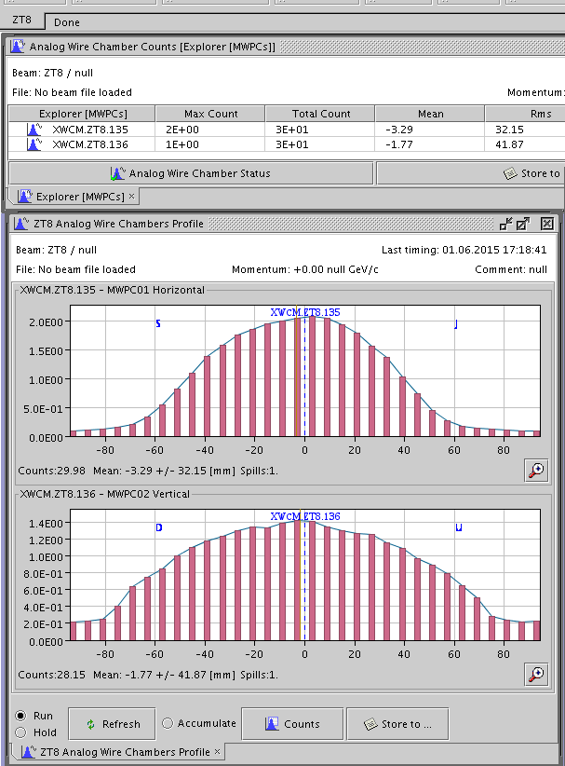
\includegraphics[width=0.6\textwidth]{./images/blown_up_beam}
	\caption{A screen-shot of the CESAR tool, showing the MWPC profile during the 'blown-up' beam reference conditions.}
	\label{fig:beam_reference2}
\end{figure}

\begin{figure}[!ht]
	\centering
	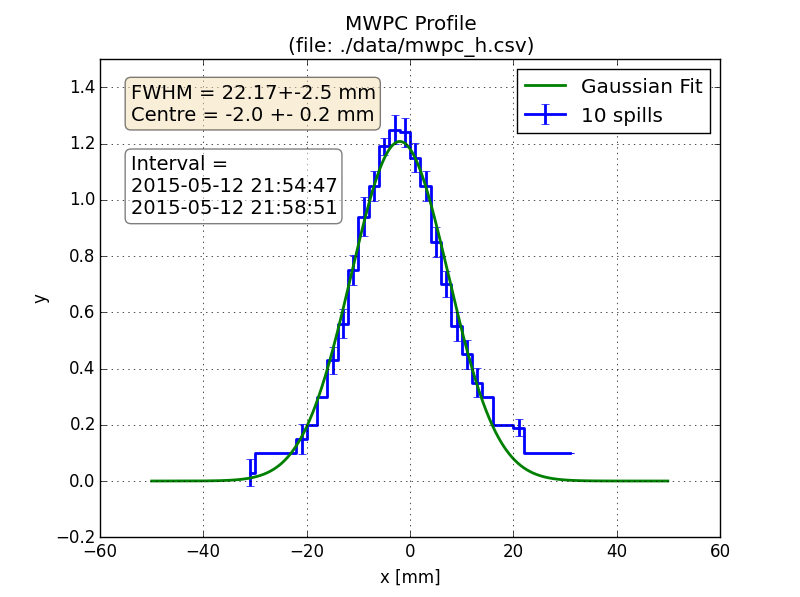
\includegraphics[width=0.6\textwidth]{./images/mwpc_com_10spills}
	\caption{A plot of the horizontal beam profile captured with the MWPC during the commissioning period. This is the typical beam used with the target.}
	\label{fig:mwpc_profile}
\end{figure}

\begin{figure}[!ht]
	\centering
	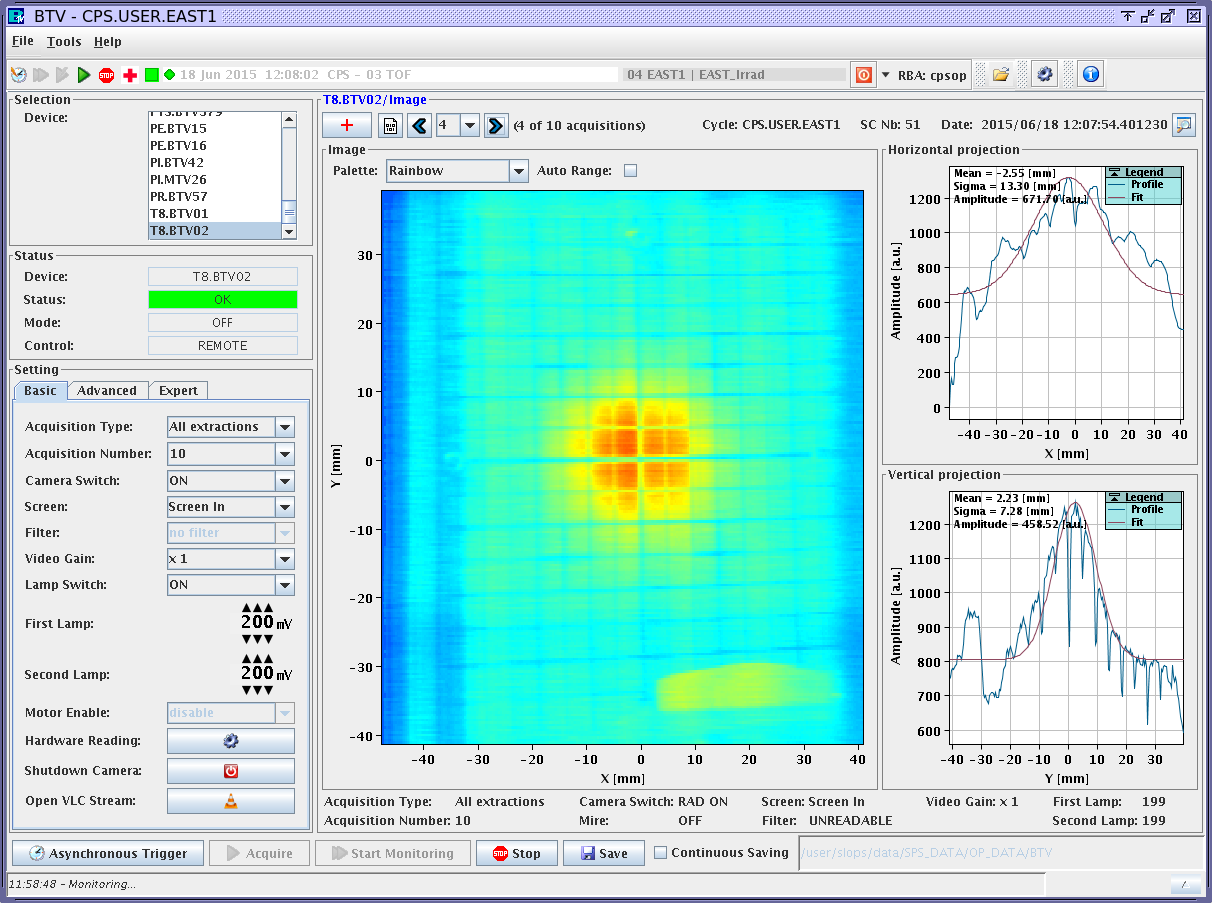
\includegraphics[width=0.5\textwidth]{./images/btv_example}
	\caption{An example of the BTV acquisition from the PS operators showing the spill alignment. In this case, the beam was aligned perfectly.}
	\label{fig:btv_example}
\end{figure}

\begin{figure}[!ht]
	\centering
	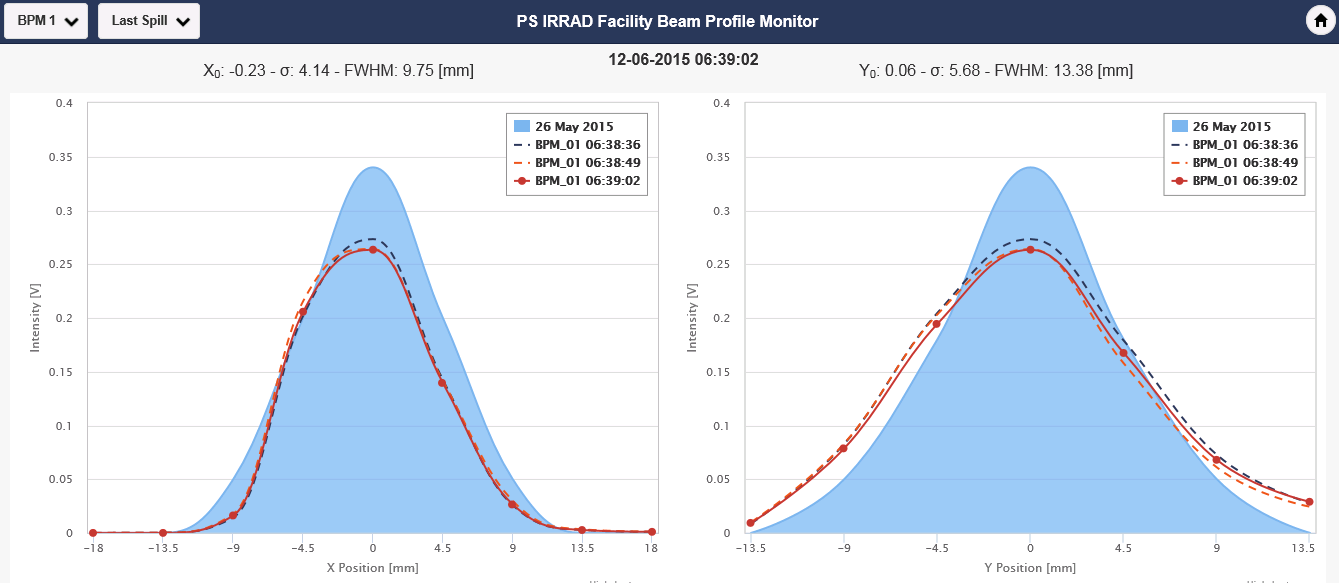
\includegraphics[width=0.8\textwidth]{./images/bpm_example}
	\caption{Example plots of the BPM1 from a typical testing period. The BPM1 is the reference when aligning the beam before using the target.}
	\label{fig:bpm_example}
\end{figure}

\begin{figure}[!ht]
	\centering
	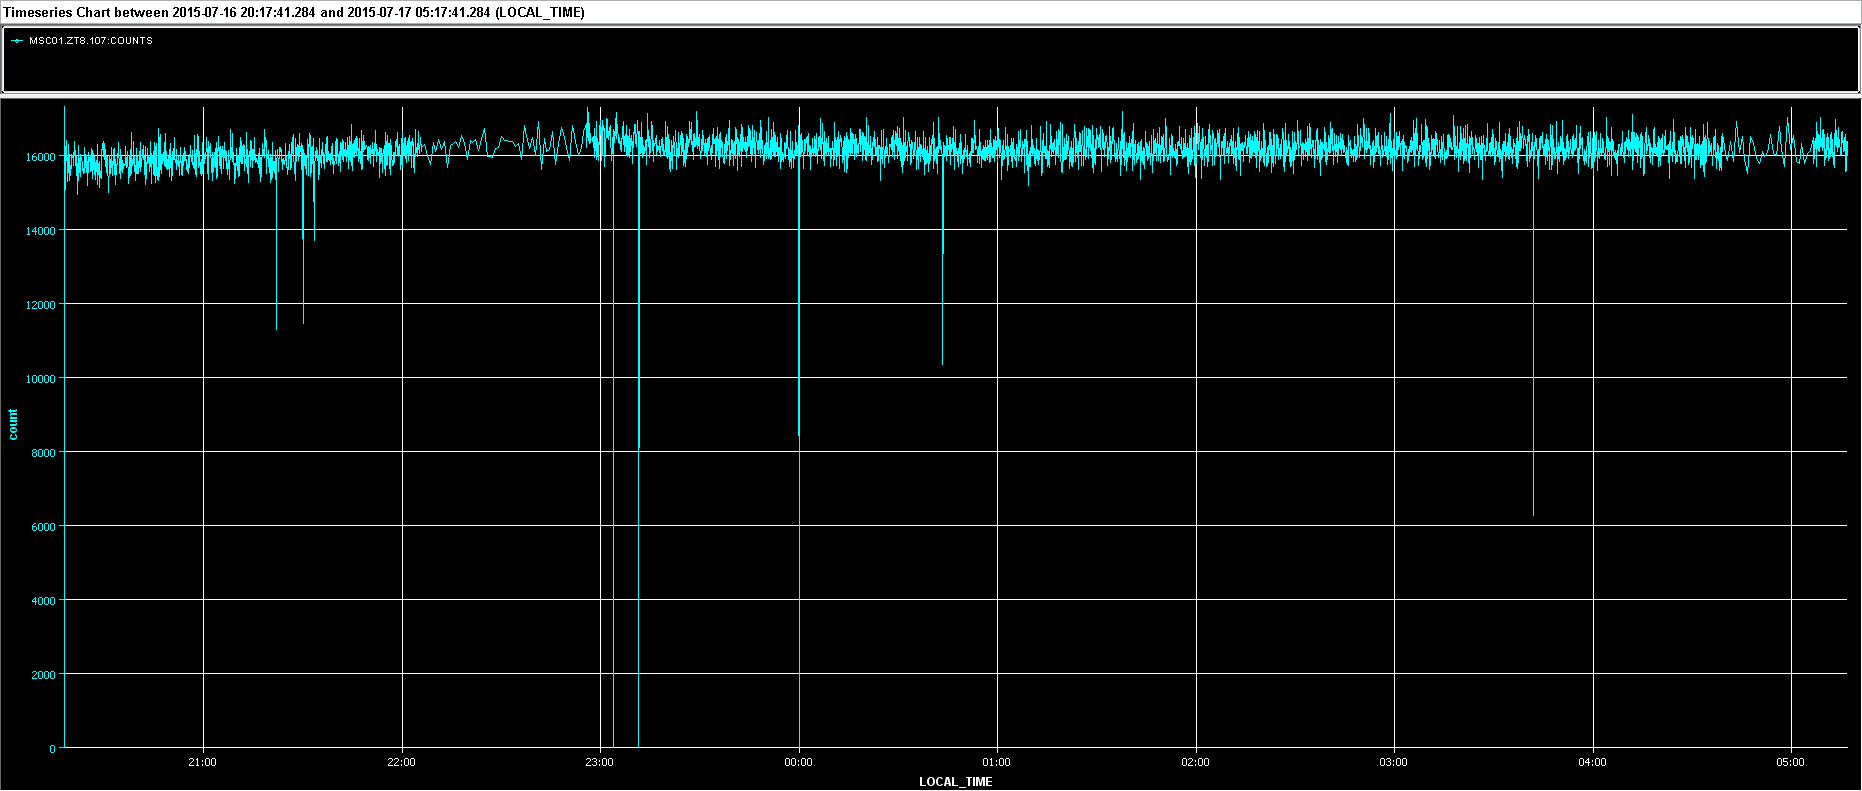
\includegraphics[width=0.8\textwidth]{./images/sec1_example}
	\caption{An example of the SEC1 signal acquired from TIMBER showing the beam intensity over a certain period.}
	\label{fig:sec_example}
\end{figure}